\documentclass[10pt]{beamer}
% \documentclass[handout,10pt]{beamer}
\usepackage{my_style}


\title[Math/CS 375]{Lecture 04 - C}
\subtitle{\S 3.3 Secant Method}

\begin{document}
% -------------------------------------------------
\begin{frame}
  \titlepage
\end{frame}
% -------------------------------------------------
\begin{frame}{Goals}
We will answer the following questions:\\[3mm]
\begin{itemize}
    \item What is the secant method?
    \item How fast does the secant method converge?
    \item What are the relative advantages and disadvantages of the bisection, Newton, and secant methods?
\end{itemize}
\end{frame}
%%%%%%%%%%%%%%%%%%%%%%%%%%%%%%%%
\sectionframe{Secant Method}
%%%%%%%%%%%%%%%%%%%%%%%%%%%%%%%%

\begin{frame}{Drawback to Newton's Method}

\begin{block}{Newton Formula}
\[
x_{k+1}
\;=\;
x_k\;-\underbrace{\frac{f(x_k)}{f'(x_k)}}_{\text{need derivative}}
\]
\end{block}

\vfill

\textbf{Pro:}
\begin{itemize}
    \item Very fast convergence near a simple root ($r=2$)
\end{itemize}

\vfill

\textbf{Con:}
\begin{itemize}
    \item Requires evaluating the derivative $f'(x)$
    \item Derivatives can be difficult or expensive to compute
    \item In higher dimensions, $f'(x)$ becomes the Jacobian matrix
\end{itemize}

\vfill

\question{
Can we approximate the derivative instead?
}

\end{frame}
% ---------------

\begin{frame}{Approximating the Derivative}

\begin{itemize}
    \item  Recall the definition of the derivative:
\[
f'(x)
=
\lim_{h\to0}
\frac{f(x+h)-f(x)}{h}.
\]

\vfill

\item This ratio is called the \textbf{difference quotient} (DQ)
\[
f'(x) \approx \frac{f(x+h)-f(x)}{h}
\]

\vfill

\item Here is an alternate equivalent DQ using two points $x$ and $y$,
\[
\boxed{
f'(x)
\approx
\frac{f(x)-f(y)}{x-y}
}
\]
\end{itemize}
\end{frame}

% ----------------------
\begin{frame}{Difference Quotient}{Let $y\to x$}

\begin{center}
\begin{tikzpicture}

\begin{axis}[
    width=10cm,
    height=6cm,
    axis lines=middle,
    xmin=0, xmax=4.5,
    ymin=-1, ymax=5,
    xlabel={$x$},
    ylabel={$f(x)$},
    xtick=\empty,
    ytick=\empty,
    samples=100,
    clip=false
]

% Function
\addplot[
    blue,
    thick,
    domain=0.5:4.2
]
{0.5*(x-1)^2};

% Fixed point x = 2
\addplot[
    only marks,
    mark=*,
    mark size=2pt
]
coordinates {(2,0.5)};

\node[below] at (axis cs:2,0) {$x$};

% ------------------------------------------------
% y = 4
% ------------------------------------------------
\only<1>{

\addplot[
    only marks,
    mark=*,
    mark size=2pt
]
coordinates {(4,4.5)};

\node[below] at (axis cs:4,0) {$y$};

% Secant slope = (4.5-.5)/(4-2) = 2
\addplot[
    red,
    thick,
    domain=1.3:4.2
]
{0.5 + 2*(x-2)};

}

% ------------------------------------------------
% y = 3
% ------------------------------------------------
\only<2>{

\addplot[
    only marks,
    mark=*,
    mark size=2pt
]
coordinates {(3,2)};

\node[below] at (axis cs:3,0) {$y$};

% Secant slope = (2-.5)/(3-2) = 1.5
\addplot[
    red,
    thick,
    domain=1.2:3.8
]
{0.5 + 1.5*(x-2)};

}

% ------------------------------------------------
% y = 2.5
% ------------------------------------------------
\only<3>{

\addplot[
    only marks,
    mark=*,
    mark size=2pt
]
coordinates {(2.5,1.125)};

\node[below] at (axis cs:2.5,0) {$y$};

% Secant slope = (1.125-.5)/(.5) = 1.25
\addplot[
    red,
    thick,
    domain=1.1:3.6
]
{0.5 + 1.25*(x-2)};

}

% ------------------------------------------------
% y = 2.2
% ------------------------------------------------
\only<4>{

\addplot[
    only marks,
    mark=*,
    mark size=2pt
]
coordinates {(2.2,0.72)};

\node[below] at (axis cs:2.2,0) {$y$};

% Secant slope = (0.72-.5)/(.2) = 1.1
\addplot[
    red,
    thick,
    domain=1.0:3.5
]
{0.5 + 1.1*(x-2)};

}

% ------------------------------------------------
% Limit: tangent at x
% f'(2) = 1
% ------------------------------------------------
\only<5>{

\addplot[
    red,
    thick,
    domain=1.0:3.5
]
{0.5 + (x-2)};

\node[red, above] at (axis cs:3.1,1.7)
    {tangent line};

}

\end{axis}

\end{tikzpicture}
\end{center}

\only<1-4>{
\[
\frac{f(x)-f(y)}{x-y}
=
\text{slope of the secant line}
\]
}

\only<5>{
\[
\boxed{
\lim_{y\to x}
\frac{f(x)-f(y)}{x-y}
=
f'(x)
}
\]
}

\end{frame}

% -----------------

\begin{frame}{Iterations}

\begin{itemize}
\item[\textbf{1.}] Suppose you have a sequence $x_k$ that converges to $x^*$\\
$$
x_k,\; x_{k+1}, \; x_{k+2},\;\dots ,\; x^*
$$
\item[\textbf{2.}] Suppose you keep $f(x_{k-1})$ in memory as you compute $f(x_k)$
\[
\underbrace{(x_{k-1},f(x_{k-1}))}_{\text{saved}} 
\qquad\text{and}\qquad
\underbrace{(x_k,f(x_k))}_{\text{newly computed}}.
\]

\vfill

\item You will always have access to a derivative approximation
\[
f'(x_k)
\approx
\frac{f(x_k)-f(x_{k-1})}
     {x_k-x_{k-1}}.
\]

\vfill
\end{itemize}

\keyidea{
As long as you save $x_{k-1}$ and $f(x_{k-1})$, approximating $f'(x_k)$ is nearly free.
}
\end{frame}

% -------

\begin{frame}{Secant Method}
\begin{itemize}
    \item[1.] Save the values of $x_{k-1}$ and $f(x_{k-1})$
    \item[2.] Instead of doing the Newton iteration
    \begin{equation*}
        x_{k+1} = x_k - \frac{f(x_k)}{f'(x_k)},
    \end{equation*}

    % \item Consider three stages 
    % \begin{align*}
    %     x_{k+1} &= \mathrm{new\ guess}\\
    %     x_k     &= \mathrm{current\ guess}\\
    %     x_{k-1} &= \mathrm{old\ guess}
    % \end{align*}

    replace $f'(x_k)$ with the approximation
    \begin{equation*}
        f'(x_k) \approx \frac{f(x_k) - f(x_{k-1})}{x_k - x_{k-1}}
    \end{equation*}

\begin{block}{Secant Method Formula}
    
    Begin with two initial guesses $x_0$, $x_1$. Update the guess with the recurrence equation:
    \begin{equation*}
        x_{k+1} = x_k - f(x_k) \left[ \frac{x_k - x_{k-1}}{f(x_k) - f(x_{k-1})} \right]
    \end{equation*}
\end{block}

\end{itemize}
\end{frame}




%%%%%%%%%%%%%%%%%%%%%%%%%%%%%%%%%%%%%%%%%%%%%%%%%%%%%%%%%%%%%%%%%%%%%%%%
\begin{frame}[fragile]{Secant Method Algorithm}

\method{Secant Method}{$f(x)$, two initial guesses $x_0$, $x_1$}
{Approximate solution to $f(x)=0$}
{Similar to Newton but the derivative is not required.}

\vspace{4mm}
Algorithm:
\begin{lstlisting}[mathescape,caption=,label=algo:secant]
initialize:  $x_0$, $x_1$                   
for $k=1,2,3\ldots$                                           
    $x_{k+1} = x_k - f(x_k) (x_k - x_{k-1})/(f(x_k) - f(x_{k-1}) )$  
    if converged, stop       
end
\end{lstlisting}
\end{frame}
%%%%%%%%%%%%%%%%%%%%%%%%%%%%%%%%%%%%%%%%%%%%%%%%%%%%%%%%%%%%%%%%%%%%%%%%

\begin{frame}{Geometric Interpretation}

\begin{center}
	\pgfimage[height=4cm]{./figs/secant}
\end{center}

There is a geometric interpretation to secant method
\begin{itemize}
    \item Draw a secant line
    \item Find the root of the secant line
    \item Repeat
\end{itemize}
\end{frame}


%%%%%%%%%%%%%%%%%%%%%%%%%%%%%%%%%%%%%%%%%%%%%%%%%%%%%%%%%%%%%%%%%%%%%%%%
\begin{frame}{Secant Method}{Geometric Interpretation}

\begin{center}
\begin{tikzpicture}

\begin{axis}[
    width=10cm,
    height=6cm,
    axis lines=middle,
    xmin=0.7, xmax=2.2,
    ymin=-1.5, ymax=2.5,
    xlabel={$x$},
    ylabel={$f(x)$},
    xtick=\empty,
    ytick=\empty,
    samples=100,
    clip=false
]

% ================================================================
% FUNCTION
% f(x) = x^2 - 2
% ================================================================
\addplot[
    blue,
    thick,
    domain=0.8:2.1
]
{x^2-2};

\node[blue, right] at (axis cs:1.8,1.0) {$f(x)$};


% ================================================================
% FIRST VIEW: INITIAL PAIR
% ================================================================
\only<1>{

% x0 = 1
\addplot[
    dashed
]
coordinates {(1,0) (1,-1)};

\addplot[
    only marks,
    mark=*,
    mark size=2pt
]
coordinates {(1,-1)};

\node[above] at (axis cs:1,0) {$x_0$};


% x1 = 2
\addplot[
    dashed
]
coordinates {(2,0) (2,2)};

\addplot[
    only marks,
    mark=*,
    mark size=2pt
]
coordinates {(2,2)};

\node[below] at (axis cs:2,0) {$x_1$};

}


% ================================================================
% SECOND VIEW: SECANT THROUGH x0 AND x1
% ================================================================
\only<2>{

% x0
\addplot[
    dashed
]
coordinates {(1,0) (1,-1)};

\addplot[
    only marks,
    mark=*,
    mark size=2pt
]
coordinates {(1,-1)};

\node[above] at (axis cs:1,0) {$x_0$};


% x1
\addplot[
    dashed
]
coordinates {(2,0) (2,2)};

\addplot[
    only marks,
    mark=*,
    mark size=2pt
]
coordinates {(2,2)};

\node[below] at (axis cs:2,0) {$x_1$};


% Secant through (1,-1) and (2,2)
% slope = 3
\addplot[
    red,
    thick,
    domain=0.9:2.05
]
{3*x-4};


% x2 = 4/3
\addplot[
    only marks,
    red,
    mark=*,
    mark size=2pt
]
coordinates {(1.333333,0)};

\node[red, above] at (axis cs:1.333333,0)
    {$x_2$};

}


% ================================================================
% THIRD VIEW: SECANT THROUGH x1 AND x2
% ================================================================
\only<3>{

% x1 = 2
\addplot[
    dashed
]
coordinates {(2,0) (2,2)};

\addplot[
    only marks,
    mark=*,
    mark size=2pt
]
coordinates {(2,2)};

\node[below] at (axis cs:2,0) {$x_1$};


% x2 = 4/3
% f(x2) = -2/9
\addplot[
    dashed
]
coordinates {(1.333333,0) (1.333333,-0.222222)};

\addplot[
    only marks,
    mark=*,
    mark size=2pt
]
coordinates {(1.333333,-0.222222)};

\node[above left] at (axis cs:1.333333,0)
    {$x_2$};


% Secant through x1 and x2
% slope = 10/3
% line: y = (10/3)x - 14/3
\addplot[
    red,
    thick,
    domain=1.2:2.05
]
{(10/3)*x - 14/3};


% x3 = 7/5
\addplot[
    only marks,
    red,
    mark=*,
    mark size=2pt
]
coordinates {(1.4,0)};

\node[red, above right] at (axis cs:1.4,0)
    {$x_3$};

}

\end{axis}

\end{tikzpicture}
\end{center}


% ================================================================
% TEXT BELOW FIGURE
% ================================================================


\only<1>{
$$
\text{1. Start with a bracket } [x_0,x_1]
$$
}

\only<2>{
\[
\text{2. Draw a  line through }
(x_0,f(x_0))
\text{ and }
(x_1,f(x_1)).
\]
$$
\text{3. Find the root of the secant line.}
$$
}
\only<3>{
\[
\text{4. Repeat with new pair}
(x_1,f(x_1))
\text{ and }
(x_2,f(x_2)).
\]
}

\end{frame}


%%%%%%%%%%%%%%%%%%%%%%%%%%%%%%%%%%%%%%%%%%%%%%%%%%%%%%%%%%%%%%%%%%%%%%%%
\begin{frame}{Hand Calculation}
\begin{example}
    Do one iteration of Newton's Method and the Secant method for the function
    $$
    f(x)=x^2-3x+1.
    $$
    Use $x_0=1$ for Newton, and use $x_0=1$, $x_1 = 5$ for Secant. 
\end{example}
Newton: 
\begin{itemize}
    \item First find the derivative: $f'(x)= 2x-3$
    \item One iteration 
    $$
    x_1 = x_0-\frac{f(x_0)}{f'(x_0)} = 1 - \frac{-1}{-5} = \frac{6}{5}.
    $$    
\end{itemize}
Secant
\begin{itemize}
    \item One iteration 
    $$
    x_2 = x_1-f(x_0)\frac{x_1-x_0}{f(x_1)-f(x_0)} = 1 - (-1)\frac{5-1}{11+1} = 1+\frac{1}{3}=\frac{4}{3}.
    $$    
\end{itemize}
\end{frame}

%%%%%%%%%%%%%%%%%%%%%%%%%%%%%%%%%%%%%%%%%%%%%%%%%%%%%%%%%%%%%%%%%%%%%%%%
\sectionframe{Error Analysis}
%%%%%%%%%%%%%%%%%%%%%%%%%%%%%%%%%%%%%%%%%%%%%%%%%%%%%%%%%%%%%%%%%%%%%%%%
\begin{frame}{Convergence Rate}

\begin{itemize}

\begin{block}{Goal}
Determine the convergence order $r$ satisfying
\[
|e_{k+1}|
\approx
C|e_k|^r.
\]
\end{block}

\item We will use the following theorem
\begin{theorem}
    The error $e_k = x_* - x_k$ for secant method satisfies 
        $$ e_{k+1} = -\frac{1}{2} \left( \frac{f''(\xi_n)}{f'(\zeta_n)} \right) e_k e_{k-1}$$
We will not prove this. See book NMC7 pg. 144
\end{theorem}
\vspace{5mm}
    \item We can simplify the theorem
    $$
    |e_{k+1}| = K|e_k||e_{k-1}|
    $$
\end{itemize}

\end{frame}


\begin{frame}{Finding the Convergence Order}{Part 1}

\begin{itemize}
\item[1.] Suppose the Secant Method has convergence order $r$:
\[
|e_{k+1}|
\approx
C|e_k|^r.
\]

\item[2.] Then one iteration earlier,
\[
|e_k|
\approx
C|e_{k-1}|^r.
\]

\item[3.] Solving for the older error gives
\[
|e_{k-1}|
\approx
\left(\frac{|e_k|}{C}\right)^{1/r}.
\]


\item[4.]<2->Substitute old error into the theorem equation
\[
|e_{k+1}|
=
K|e_k||e_{k-1}| 
\]
to obtain 
\[
|e_{k+1}|
\approx
K C^{-1/r}
|e_k|^{\,1+1/r}.
\]

\end{itemize}
\end{frame}


%%%%%%%%%%%%%%%%%%%%%%%%%%%%%%%%%%%%%%%%%%%%%%%%%%%%%%%%%%%%%%%%%%%%%%%%
\begin{frame}{Finding the Convergence Order}{Part 2}

\begin{itemize}

    \item[5.] Compare the two expressions for the new error:
    \[
    |e_{k+1}|
    \approx
    C|e_k|^{\textcolor{red}{r}}
    \qquad \text{vs.} \qquad
    |e_{k+1}|
    \approx
    K C^{-1/r}|e_k|^{\textcolor{red}{1+1/r}}.
    \]
    For these to be consistent, the powers of $|e_k|$ must agree:
    \[
    r=1+\frac{1}{r}.
    \]

    \item<2->[6.] Multiply by $r$ and rearrange:
    \[
    r^2-r-1=0.
    \]

    \item<3->[7.] Solve using the quadratic formula to obtain the convergence rate
    \[
    \boxed{
    r=\frac{1+\sqrt{5}}{2}\approx1.618
    }
    \]
    where we discard the negative root.


\end{itemize}

\end{frame}

% -----------------------------

\begin{frame}{Superlinear Convergence}

\begin{itemize}
    \item This quantity is called the \textbf{golden ratio}
    \[
    r=\frac{1+\sqrt{5}}{2}\approx1.618
    \]
    \item Convergence rate for secant is \textit{between} linear and quadratic 
    $$
        \underbrace{1}_{\text{linear}} < 1.618 < \underbrace{2}_{\text{quadratic}}
    $$
    \item We call this \textbf{superlinear} convergence
\end{itemize}

\keyidea{
Secant is faster than bisection but slower than Newton.
}
    
\end{frame}

%%%%%%%%%%%%%%%%%%%%%%%%%%%%

\begin{frame}{Experimental Approach}

\begin{block}{Make a Table}
    
\begin{enumerate}
    \item Calculate a sequence of errors $e_0$, $e_1$, $\dots$, $e_k$,$\dots$

    \item Calculate a table of error ratios with $k$ and $e^{k+1}/e_{k}^r$

    \item Numbers should be roughly constant
\end{enumerate}
\end{block}


\begin{block}{Formula}
\begin{itemize}
    \item Assume $e_{k+1}\approx Ce_{k}^r$
    \item Then $e_{k}\approx Ce_{k-1}^r$
    \item Divide 
    $$
     \frac{e_{k+1}}{e_k} \approx \left(\frac{e_k}{e_{k-1}}\right)^r
    $$
    \item Solve for $r$
\end{itemize}

    
\end{block}

    

    
\end{frame}

%%%%%%%%%%%%%%%%%%%%%%%%%%%%%%%%%%%%%%%%%%%%%%%%%%%%%%%%%%%%%%%%%%%%%%%
\sectionframe{Comparison of Rootfinding Methods}
%%%%%%%%%%%%%%%%%%%%%%%%%%%%%%%%%%%%%%%%%%%%%%%%%%%%%%%%%%%%%%%%%%%%%%%

\begin{frame}{Revisit Example}


    \begin{block}{Problem}
    Consider finding the root of 
        \begin{equation*}
   f(x) = x - x^{1/3} - 2 = 0
\end{equation*}
    using bisection, Newton's method, and Secant method. How many iterations does each one require to get machine precision?
    \end{block}

\end{frame}

\begin{frame}{Revisit Example}{Bisection}

\textbf{Bisection:}
\begin{center}
  \small
  \renewcommand{\arraystretch}{1.3}
    \begin{tabular}{clllr}
     $k$ & \multicolumn{1}{c}{$a$}
         & \multicolumn{1}{c}{$b$}
         & \multicolumn{1}{c}{$x_{mid}$}
         & \multicolumn{1}{c}{$f(x_{mid})$} \\ \hline
      1 & 3.00000000 & 4.00000000 & 3.50000000 & -0.01829449 \\
      2 & 3.50000000 & 4.00000000 & 3.75000000 &  0.19638375 \\
      3 & 3.50000000 & 3.75000000 & 3.62500000 &  0.08884159 \\
      4 & 3.50000000 & 3.62500000 & 3.56250000 &  0.03522131 \\
      5 & 3.50000000 & 3.56250000 & 3.53125000 &  0.00845016 \\
      6 & 3.50000000 & 3.53125000 & 3.51562500 & -0.00492550 \\
      7 & 3.51562500 & 3.53125000 & 3.52343750 &  0.00176150 \\
      8 & 3.51562500 & 3.52343750 & 3.51953125 & -0.00158221 \\
      9 & 3.51953125 & 3.52343750 & 3.52148438 &  0.00008959 \\
     10 & 3.51953125 & 3.52148438 & 3.52050781 & -0.00074632
    \end{tabular}
\end{center}

\vfill

\begin{center}
\[
\vdots
\]
At iteration $51$, $\operatorname{fl}(f(x_{mid}))=0$.
\end{center}

\end{frame}


\begin{frame}{Revisit Example}{Newton and Secant}
\textbf{Newton}
\begin{center}
  \small
    \renewcommand{\arraystretch}{1.3}
    \begin{tabular}{cccc}
    $k$ &    $x_k$     & $f'(x_k)$  &   $f(x)$                   \\ \hline
     0  &  3           & 0.83975005 & -0.44224957                \\
     1  &  3.52664429  & 0.85612976 &  0.00450679                \\
     2  &  3.52138015  & 0.85598641 &  $3.771\times 10^{-7}$   \\
     3  &  3.52137971  & 0.85598640 &  $2.664\times 10^{-15}$ \\
     4  &  3.52137971  & 0.85598640 &  0.0                       \\
    \end{tabular}
\end{center}
\textbf{Secant}
\begin{center}
  \small
    \begin{tabular}{cccc}
       $k$ &   $x_{k-1}$  &    $x_k$   & $f(x_k)$                  \\ \hline
        0  &  4           & 3          & $-0.44224957$               \\
        1  &  3           & 3.51734262 & $-0.00345547$               \\
        2  &  3.51734262  & 3.52141665 & $0.00003163 $              \\
        3  &  3.52141665  & 3.52137970 & $-2.034\times 10^{-9}$  \\
        4  &  3.52137959  & 3.52137971 & $-1.332\times 10^{-15}$ \\
        5  &  3.52137971  & 3.52137971 &  0.0                      \\
        \end{tabular}
\end{center}
\end{frame}

\begin{frame}{Comparison}
\begin{figure}
    \centering
    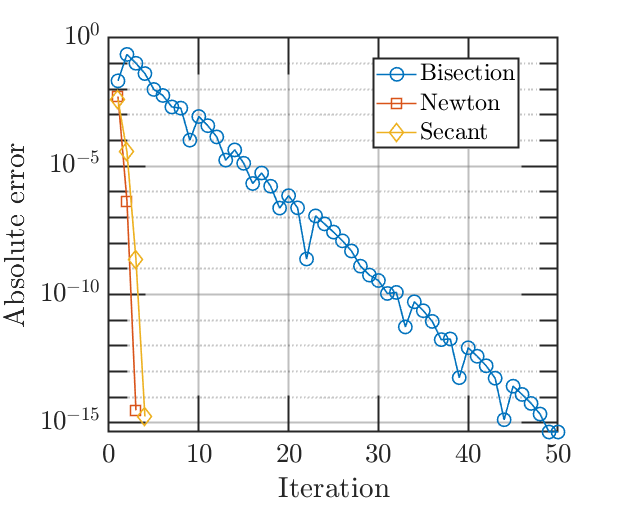
\includegraphics[width=0.55\linewidth]{figs/rootfinding.png}
\end{figure}

\begin{itemize}
    \item Bisection requires many more iterations
    \item Newton and Secant reach machine precision very quickly
\end{itemize}

\vfill

\question{
If Bisection is so much slower, why would we ever use it?
}
\end{frame}

\begin{frame}{Comparison of Rootfinding Methods}

\begin{center}
\renewcommand{\arraystretch}{1.5}
\begin{tabular}{c|c|c|c}
 & Bisection & Newton & Secant \\ \hline
Convergence
    & Linear
    & Quadratic
    & Superlinear \\

Rate $r$
    & $1$
    & $2$
    & $\approx 1.618$ \\

Derivative
    & No
    & Yes
    & No \\

Initial values
    & $2$
    & $1$
    & $2$ \\

Guaranteed
    & Yes*
    & No
    & No
\end{tabular}
\end{center}

\vfill

{\small *Assuming $f$ is continuous and the initial interval brackets a root.}

\vfill

\keyidea{
There is no best rootfinding method. Each has different
advantages and disadvantages.
}

\end{frame}





%%%%%%%%%%%%%%%%%%%%%%%%%%%%%%%%%%%%%%%%%%%%%%%%%%%%%%%%%%%%%%%%%%%%%%%%
\sectionframe{Extra Topic: Modern Root-finding}
%%%%%%%%%%%%%%%%%%%%%%%%%%%%%%%%%%%%%%%%%%%%%%%%%%%%%%%%%%%%%%%%%%%%%%%%
\begin{frame}{Two Ideas}

\begin{block}{Idea 1}
    Make an algorithm that uses a combination of bisection, secant, and Newton's method so that it is both fast and reliable.  - \textbf{Brent's method}
\end{block}
\bigskip

\begin{block}{Idea 2}
    Make an algorithm that is able to find complex roots and handle roots with multiple zeros. - \textbf{companion matrix method}
\end{block}
    
\end{frame}

%%%%%%%%%%%%%%%%%%%%%%%%%%%%%%%%%%%%%%%%%%%%%%%%%%%%%%%%%%%%%%%%%%%%%%%%

\begin{frame}{When Secant Can Fail}

\begin{center}
    \pgfimage[height=4.5cm]{./figs/secantFails}
\end{center}

\begin{itemize}

    \item Recall the Secant update:
    \[
    x_{k+1}
    =
    x_k
    -
    f(x_k)
    \frac{x_k-x_{k-1}}
         {f(x_k)-f(x_{k-1})}.
    \]

    \item<2-> Problem when 
    \[
    \frac{f(x_k)-f(x_{k-1})}
         {x_k-x_{k-1}}
    \approx 0,
    \]

\end{itemize}
\end{frame}

% ------------

\begin{frame}{Can We Make Secant Safer?}

\begin{center}
    \pgfimage[height=4cm]{./figs/secantFails}
\end{center}

\begin{itemize}
    \item Bisection always preserves a bracket 

    \item<2-> Secant can leave the bracket and potentially diverge
\end{itemize}

\vfill


\onslide<3->{
\question{
Can we get the speed of Secant with the reliability of Bisection?
}
}

\end{frame}


%%%%%%%%%%%%%%%%%%%%%%%%%%%%%%%%%%%%%%%%%%%%%%%%%%%%%%%%%%%%%%

\begin{frame}[fragile]{Idea 1: \texttt{fzero} Function}


\begin{block}{Brent's Method}
    
\textbf{Brent's Method} uses a hybrid rootfinding algorithm that combines
\textbf{bisection}, \textbf{secant}, and
\textbf{inverse quadratic interpolation}.
\end{block}


\vspace{3ex}
In Matlab, use the built-in function \texttt{fzero()}
\begin{lstlisting}[language=matlab]
r = fzero(fun,x0)
r = fzero(fun,x0,options)
\end{lstlisting}

\vspace{3ex}

\texttt{x0} can be a scalar or a two-element vector:
\begin{itemize}
    \item If \texttt{x0} is a scalar, \texttt{fzero} searches
          for a bracket containing a sign change.

    \item If \texttt{x0} is a two-element vector, it must
          bracket a sign change.
\end{itemize}

\end{frame}
%%%%%%%%%%%%%%%%%%%%%%%%%%%%%%%%%%%%%%%%%%%%%%%%%%%%%%%%%%%%%%%%%%%%%%%%
\begin{frame}{Inverse Quadratic Interpolation}

\begin{itemize}
    \item Start with 3 points 
\[
(x_0,f(x_0)),\qquad
(x_1,f(x_1)),\qquad
(x_2,f(x_2)).
\]
\item Approximate $f$ with a \textbf{sideways parabola}
\item New point $x_3$ is the root of the parabola
\end{itemize}

\begin{center}
    \pgfimage[height=4.8cm]{./figs/fzeroPicture2}
\end{center}

\end{frame}

%%%%%%%%%%%%%%%%%%%%%%%%%%%%%%%%%%%%%%%%%%%%%%%%%%%%%%%%%%%%%%%%%%%%%%%%

\begin{frame}{\texttt{fzero}: A Hybrid Method}


At each iteration, \texttt{fzero} can use:
\begin{itemize}

    \item \textbf{Inverse quadratic interpolation}
    when three suitable points are available.

    \item<2-> \textbf{Secant interpolation}
    when two suitable points are available.

    \item<3-> \textbf{Bisection}
    when an interpolation step is not considered safe.

\end{itemize}

\vfill

\onslide<4->{
\keyidea{
Use fast interpolation when possible, but use Bisection
to safeguard the search.
}
}


\end{frame}

%%%%%%%%%%%%%%%%%%%%%%%%%%%%%%%%%%%%%%%%%%%%%%%%%%%%%%%%%%%%%%%%%%%%%%%%

\begin{frame}[fragile]{\texttt{fzero} Function}



Command \texttt{fzero} finds the root closest to the initial point
\begin{lstlisting}[language=matlab]
>> x = fzero(@cos,0.5)
x =
    1.5708
\end{lstlisting}


\vfill 
Use \texttt{optimset} to create settings 
\begin{lstlisting}[language=matlab]
>> options = optimset('Display','iter');
>> x = fzero(@cos, 0.5, options)
\end{lstlisting}

\vfill 
Choose the error tolerance
\vspace{0.0cm}
\begin{lstlisting}[language=matlab]
>> options = optimset('TolX',5e-9);
>> x = fzero(@cos, 0.5, options)
\end{lstlisting}
\end{frame}

% -----------------------

\begin{frame}[fragile]{Demo}
$$
   f(x) = x - x^{1/3} - 2 = 0
$$
\begin{lstlisting}[language=matlab]
f  = @(x) x - x.^(1/3) - 2;
options = optimset('Display','iter');
r = fzero(f,3,options)
\end{lstlisting}

\begin{alltt}\tiny
 
Search for an interval around 3 containing a sign change:
 Func-count    a          f(a)             b          f(b)        Procedure
    1               3      -0.44225             3      -0.44225   initial interval
    3         2.91515     -0.513374       3.08485     -0.370868   search
    5            2.88     -0.542757          3.12     -0.341229   search
    7         2.83029      -0.58423       3.16971     -0.299242   search
    9            2.76     -0.642716          3.24     -0.239727   search
   11         2.66059     -0.725079       3.33941     -0.155298   search
   13            2.52     -0.840818          3.48     -0.035397   search
   15         2.32118      -1.00287       3.67882      0.135099   search
 
Search for a zero in the interval [2.32118, 3.67882]:
 Func-count    x          f(x)             Procedure
   15         3.67882      0.135099        initial
   16         3.51764   -0.00319777        interpolation
   17         3.52137  -7.81109e-06        interpolation
   18         3.52138   1.34328e-11        interpolation
   19         3.52138             0        interpolation
 
Zero found in the interval [2.32118, 3.67882]
r = 3.5214
\end{alltt}
    
\end{frame}

%%%%%%%%%%%%%%%%%%%%%%%%%%%%%%%%%%%%%%%%%%%%%%%%%%%%%%%%%%%%%%%%%%%%%%%%
\begin{frame}[fragile]{Another \texttt{fzero} example}

\question{
    How well does \texttt{fzero} handle multiple zeros?
}

\begin{itemize}
    \item Consider the polynomial
        \begin{equation*}
          f(x) = x^{10} - 1
        \end{equation*}
    \item Solution: $x=\pm 1$\\[3mm]
\begin{lstlisting}[language=matlab]
>> f = @(x)x.^10 - 1;
>>  options = optimset('display','iter');
>> [x,fx]=fzero(f,0.5,options)
\end{lstlisting}
    \item It take \underline{35 iterations}! 
\end{itemize}
\end{frame}

%%%%%%%%%%%%%%%%%%%%%%%%%%%%%%%%%%%%%%%%%%%%%%%%%%%%%%%%%%%%%%%%%%%%%%

%%%%%%%%%%%%%%%%%%%%%%%%%%%%%%%%%%%%%%%%%%%%%%%%%%%%%%%%%%%%%%%%%%%%%%
\begin{frame}[fragile]{Idea 2: \texttt{roots}}

\begin{block}{Polynomial Rootfinding}
The MATLAB function \texttt{roots} is specifically designed
to find roots of polynomials.
\end{block}

\begin{itemize}
    \item No initial guess
    \item Returns \emph{all} roots of the polynomial
    \item Can find real, repeated, and complex roots
\end{itemize}

\vspace{4ex}
Write polynomial in the form
\begin{equation*}
    c_1 x^n + c_2 x^{n-1} + \ldots + c_n x + c_{n+1} = 0
\end{equation*}
For example, for a cubic polynomial:
\begin{lstlisting}[language=matlab]
>> c = [c1 c2 c3 c4];
>> r = roots(c)
\end{lstlisting}
\end{frame}

%%%%%%%%%%%%%%%%%%%%%%%%%%%%%%%%%%%%%%%%%%%%%%%%%%%%%%%%%%%%%%%%%%%%%%%%

\begin{frame}[shrink]{\texttt{roots} - How it works}
\begin{itemize}
    \item Consider the matrix
    \begin{equation*}
        A = \begin{bmatrix} 0 & 1 & 0 & 0 \\
                            0 & 0 & 1 & 0 \\
                            0 & 0 & 0 & 1 \\
                           -c_0 & -c_1 & -c_2 & -c_3 \end{bmatrix}
    \end{equation*}
\item Find the eigenvalues by setting the determinant of $A-\lambda I$ to zero
    \begin{equation*}
    A -\lambda I= 
       \begin{bmatrix} -\lambda & 1 & 0 & 0 \\
                        0 & -\lambda & 1 & 0 \\
                        0 & 0 & -\lambda & 1 \\
                       -c_0 & -c_1 & -c_2 & (-c_3 - \lambda)\end{bmatrix}
    \end{equation*}
    \item But that is a polynomial 
    $$ \det(A-\lambda I) = p(\lambda) = \lambda^4 + c_3 \lambda^3 + c_2 \lambda^2 + c_1 \lambda + c_0 $$
    \item Use eigenvalue solvers to find roots of polynomials! 
\end{itemize}
\end{frame}

%%%%%%%%%%%%%%%%%%%%%%%%%%%%%%%%%%%%%%%%%%%%%%%%%%%%%%%%%%%%%%%%%%%%%%%%

\begin{frame}[fragile,shrink]{\texttt{roots} - Examples}

Come examples
\begin{align*}
    f_1(x) &= x^2 -  3x +  2    \qquad \text{two real roots}\\
    f_2(x) &= x^2 - 10x + 25    \qquad \text{repeated roots}\\
    f_3(x) &= x^2 - 17x + 72.5  \qquad \text{complex roots}
\end{align*}

\begin{lstlisting}[language=matlab]
>> roots([1 -3 2])
ans =
        2
        1

>> roots([1 -10 25])
ans =
        5
        5

>> roots([1 -17 72.5])
ans =
    8.5000 + 0.5000i
    8.5000 - 0.5000i
\end{lstlisting}
\end{frame}

%%%%%%%%%%%%%%%%%%%%%%%%%%%%%%%%%%%%%%%%%%%
\begin{frame}[fragile,shrink]{Degree 10 Polynomial}

\begin{align*}
    f(x) &= x^{10} - 1 = 0     \\
\end{align*}

\begin{lstlisting}[language=matlab]
>> c = [1, zeros(1,9), -1];

>> roots(c) % finds all 10 roots
ans =
  -1.0000 + 0.0000i % x=-1 found 
  -0.8090 + 0.5878i
  -0.8090 - 0.5878i
  -0.3090 + 0.9511i
  -0.3090 - 0.9511i
   0.3090 + 0.9511i
   0.3090 - 0.9511i
   1.0000 + 0.0000i % x=1 found 
   0.8090 + 0.5878i
   0.8090 - 0.5878i
\end{lstlisting}
\end{frame}



\end{document}
